% Options for packages loaded elsewhere
\PassOptionsToPackage{unicode}{hyperref}
\PassOptionsToPackage{hyphens}{url}
\PassOptionsToPackage{dvipsnames,svgnames*,x11names*}{xcolor}
%
\documentclass[
]{article}
\usepackage{lmodern}
\usepackage{amssymb,amsmath}
\usepackage{ifxetex,ifluatex}
\ifnum 0\ifxetex 1\fi\ifluatex 1\fi=0 % if pdftex
  \usepackage[T1]{fontenc}
  \usepackage[utf8]{inputenc}
  \usepackage{textcomp} % provide euro and other symbols
\else % if luatex or xetex
  \usepackage{unicode-math}
  \defaultfontfeatures{Scale=MatchLowercase}
  \defaultfontfeatures[\rmfamily]{Ligatures=TeX,Scale=1}
\fi
% Use upquote if available, for straight quotes in verbatim environments
\IfFileExists{upquote.sty}{\usepackage{upquote}}{}
\IfFileExists{microtype.sty}{% use microtype if available
  \usepackage[]{microtype}
  \UseMicrotypeSet[protrusion]{basicmath} % disable protrusion for tt fonts
}{}
\makeatletter
\@ifundefined{KOMAClassName}{% if non-KOMA class
  \IfFileExists{parskip.sty}{%
    \usepackage{parskip}
  }{% else
    \setlength{\parindent}{0pt}
    \setlength{\parskip}{6pt plus 2pt minus 1pt}}
}{% if KOMA class
  \KOMAoptions{parskip=half}}
\makeatother
\usepackage{xcolor}
\IfFileExists{xurl.sty}{\usepackage{xurl}}{} % add URL line breaks if available
\IfFileExists{bookmark.sty}{\usepackage{bookmark}}{\usepackage{hyperref}}
\hypersetup{
  pdftitle={What Makes Penguins Chonky},
  pdfauthor={Dan Ovando; Daniel Ovando},
  colorlinks=true,
  linkcolor=blue,
  filecolor=Maroon,
  citecolor=Blue,
  urlcolor=Blue,
  pdfcreator={LaTeX via pandoc}}
\urlstyle{same} % disable monospaced font for URLs
\usepackage[margin=1in]{geometry}
\usepackage{longtable,booktabs}
% Correct order of tables after \paragraph or \subparagraph
\usepackage{etoolbox}
\makeatletter
\patchcmd\longtable{\par}{\if@noskipsec\mbox{}\fi\par}{}{}
\makeatother
% Allow footnotes in longtable head/foot
\IfFileExists{footnotehyper.sty}{\usepackage{footnotehyper}}{\usepackage{footnote}}
\makesavenoteenv{longtable}
\usepackage{graphicx}
\makeatletter
\def\maxwidth{\ifdim\Gin@nat@width>\linewidth\linewidth\else\Gin@nat@width\fi}
\def\maxheight{\ifdim\Gin@nat@height>\textheight\textheight\else\Gin@nat@height\fi}
\makeatother
% Scale images if necessary, so that they will not overflow the page
% margins by default, and it is still possible to overwrite the defaults
% using explicit options in \includegraphics[width, height, ...]{}
\setkeys{Gin}{width=\maxwidth,height=\maxheight,keepaspectratio}
% Set default figure placement to htbp
\makeatletter
\def\fps@figure{htbp}
\makeatother
\setlength{\emergencystretch}{3em} % prevent overfull lines
\providecommand{\tightlist}{%
  \setlength{\itemsep}{0pt}\setlength{\parskip}{0pt}}
\setcounter{secnumdepth}{5}
\usepackage{setspace}\doublespacing
\usepackage{lineno}\linenumbers
\usepackage{booktabs}
\usepackage{longtable}
\usepackage{array}
\usepackage{multirow}
\usepackage{wrapfig}
\usepackage{float}
\usepackage{colortbl}
\usepackage{pdflscape}
\usepackage{tabu}
\usepackage{threeparttable}
\usepackage{threeparttablex}
\usepackage[normalem]{ulem}
\usepackage{makecell}
\usepackage{xcolor}
\newlength{\cslhangindent}
\setlength{\cslhangindent}{1.5em}
\newenvironment{cslreferences}%
  {\setlength{\parindent}{0pt}%
  \everypar{\setlength{\hangindent}{\cslhangindent}}\ignorespaces}%
  {\par}

\title{What Makes Penguins Chonky}
\author{Dan Ovando \and Daniel Ovando}
\date{2020-11-16}

\begin{document}
\maketitle

{
\hypersetup{linkcolor=}
\setcounter{tocdepth}{2}
\tableofcontents
}
\hypertarget{introduction}{%
\section{Introduction}\label{introduction}}

Penguins are pretty great. However, Keum \emph{et al.} (2001) showed that both fat and imaginary penguins can ``decay amplitudes in perturbative QCD picture''. Since that sounds pretty bad, we should probably figure out what makes penguins fat, if not imaginary. The mean penguin weighs 9.2632844 pounds.

Male penguins tend to be fatter than female penguins, and it looks like Gentoo penguins on Biscoe island might be at serious risk of perturbing the QCD picture (Fig.\ref{fig:weight-fig}) (Keum \emph{et al.} 2001; Horst \emph{et al.} 2020).

\begin{figure}
\centering
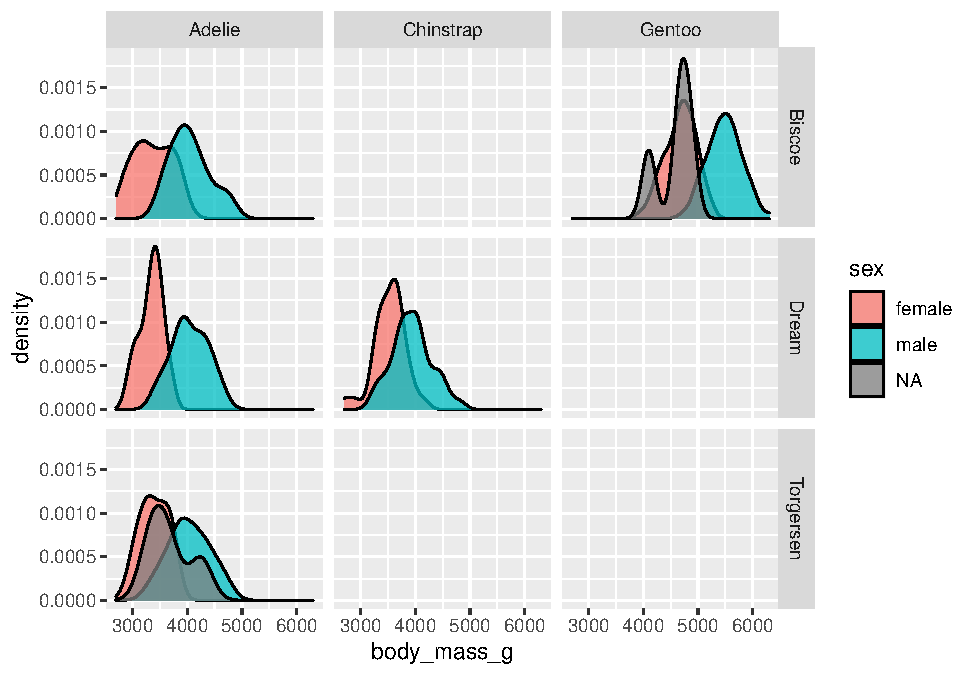
\includegraphics{my-pub_files/figure-latex/weight-fig-1.pdf}
\caption{\label{fig:weight-fig}Distribution of penguin weight in grams by sex,species, and island.}
\end{figure}

But, it seems like bill length and flipper length matter too (Fig.\ref{fig:weight-plot-2}).

\begin{figure}
\centering
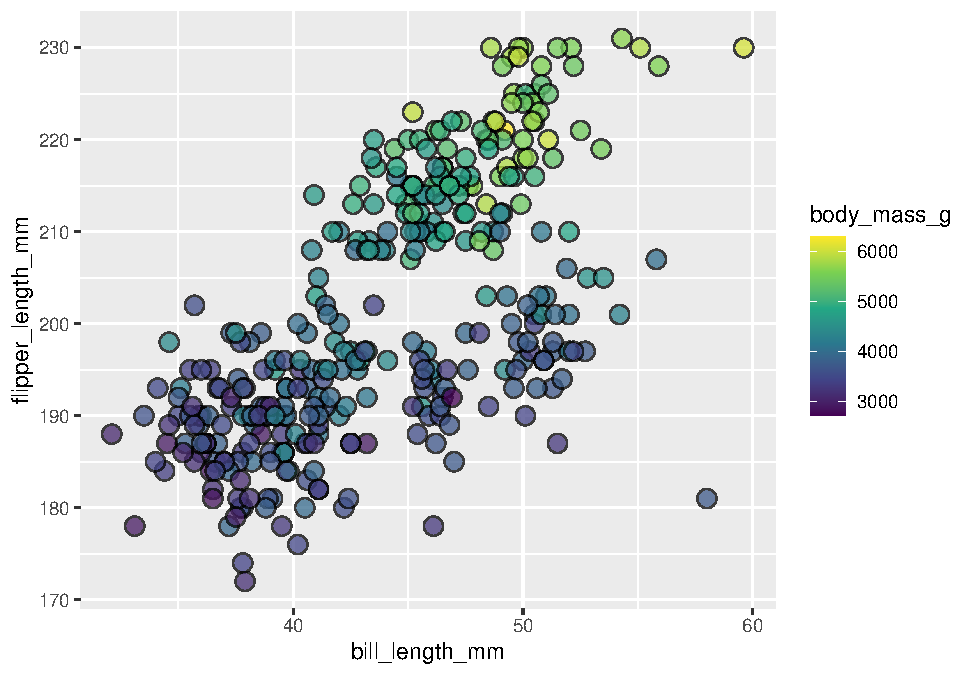
\includegraphics{my-pub_files/figure-latex/weight-plot-2-1.pdf}
\caption{\label{fig:weight-plot-2}Penguin body mass from Horst \emph{et al.} (2020) as a function of bill length and flipper length}
\end{figure}

For those that like tables, here's a table of some penguins (Table.\ref{tab:pen-tab}).

\begin{longtable}[]{@{}llrrrrlr@{}}
\caption{\label{tab:pen-tab}Here are some penguins}\tabularnewline
\toprule
\begin{minipage}[b]{0.07\columnwidth}\raggedright
species\strut
\end{minipage} & \begin{minipage}[b]{0.09\columnwidth}\raggedright
island\strut
\end{minipage} & \begin{minipage}[b]{0.13\columnwidth}\raggedleft
bill\_length\_mm\strut
\end{minipage} & \begin{minipage}[b]{0.12\columnwidth}\raggedleft
bill\_depth\_mm\strut
\end{minipage} & \begin{minipage}[b]{0.16\columnwidth}\raggedleft
flipper\_length\_mm\strut
\end{minipage} & \begin{minipage}[b]{0.11\columnwidth}\raggedleft
body\_mass\_g\strut
\end{minipage} & \begin{minipage}[b]{0.06\columnwidth}\raggedright
sex\strut
\end{minipage} & \begin{minipage}[b]{0.04\columnwidth}\raggedleft
year\strut
\end{minipage}\tabularnewline
\midrule
\endfirsthead
\toprule
\begin{minipage}[b]{0.07\columnwidth}\raggedright
species\strut
\end{minipage} & \begin{minipage}[b]{0.09\columnwidth}\raggedright
island\strut
\end{minipage} & \begin{minipage}[b]{0.13\columnwidth}\raggedleft
bill\_length\_mm\strut
\end{minipage} & \begin{minipage}[b]{0.12\columnwidth}\raggedleft
bill\_depth\_mm\strut
\end{minipage} & \begin{minipage}[b]{0.16\columnwidth}\raggedleft
flipper\_length\_mm\strut
\end{minipage} & \begin{minipage}[b]{0.11\columnwidth}\raggedleft
body\_mass\_g\strut
\end{minipage} & \begin{minipage}[b]{0.06\columnwidth}\raggedright
sex\strut
\end{minipage} & \begin{minipage}[b]{0.04\columnwidth}\raggedleft
year\strut
\end{minipage}\tabularnewline
\midrule
\endhead
\begin{minipage}[t]{0.07\columnwidth}\raggedright
Adelie\strut
\end{minipage} & \begin{minipage}[t]{0.09\columnwidth}\raggedright
Torgersen\strut
\end{minipage} & \begin{minipage}[t]{0.13\columnwidth}\raggedleft
39.1\strut
\end{minipage} & \begin{minipage}[t]{0.12\columnwidth}\raggedleft
18.7\strut
\end{minipage} & \begin{minipage}[t]{0.16\columnwidth}\raggedleft
181\strut
\end{minipage} & \begin{minipage}[t]{0.11\columnwidth}\raggedleft
3750\strut
\end{minipage} & \begin{minipage}[t]{0.06\columnwidth}\raggedright
male\strut
\end{minipage} & \begin{minipage}[t]{0.04\columnwidth}\raggedleft
2007\strut
\end{minipage}\tabularnewline
\begin{minipage}[t]{0.07\columnwidth}\raggedright
Adelie\strut
\end{minipage} & \begin{minipage}[t]{0.09\columnwidth}\raggedright
Torgersen\strut
\end{minipage} & \begin{minipage}[t]{0.13\columnwidth}\raggedleft
39.5\strut
\end{minipage} & \begin{minipage}[t]{0.12\columnwidth}\raggedleft
17.4\strut
\end{minipage} & \begin{minipage}[t]{0.16\columnwidth}\raggedleft
186\strut
\end{minipage} & \begin{minipage}[t]{0.11\columnwidth}\raggedleft
3800\strut
\end{minipage} & \begin{minipage}[t]{0.06\columnwidth}\raggedright
female\strut
\end{minipage} & \begin{minipage}[t]{0.04\columnwidth}\raggedleft
2007\strut
\end{minipage}\tabularnewline
\begin{minipage}[t]{0.07\columnwidth}\raggedright
Adelie\strut
\end{minipage} & \begin{minipage}[t]{0.09\columnwidth}\raggedright
Torgersen\strut
\end{minipage} & \begin{minipage}[t]{0.13\columnwidth}\raggedleft
40.3\strut
\end{minipage} & \begin{minipage}[t]{0.12\columnwidth}\raggedleft
18.0\strut
\end{minipage} & \begin{minipage}[t]{0.16\columnwidth}\raggedleft
195\strut
\end{minipage} & \begin{minipage}[t]{0.11\columnwidth}\raggedleft
3250\strut
\end{minipage} & \begin{minipage}[t]{0.06\columnwidth}\raggedright
female\strut
\end{minipage} & \begin{minipage}[t]{0.04\columnwidth}\raggedleft
2007\strut
\end{minipage}\tabularnewline
\begin{minipage}[t]{0.07\columnwidth}\raggedright
Adelie\strut
\end{minipage} & \begin{minipage}[t]{0.09\columnwidth}\raggedright
Torgersen\strut
\end{minipage} & \begin{minipage}[t]{0.13\columnwidth}\raggedleft
NA\strut
\end{minipage} & \begin{minipage}[t]{0.12\columnwidth}\raggedleft
NA\strut
\end{minipage} & \begin{minipage}[t]{0.16\columnwidth}\raggedleft
NA\strut
\end{minipage} & \begin{minipage}[t]{0.11\columnwidth}\raggedleft
NA\strut
\end{minipage} & \begin{minipage}[t]{0.06\columnwidth}\raggedright
NA\strut
\end{minipage} & \begin{minipage}[t]{0.04\columnwidth}\raggedleft
2007\strut
\end{minipage}\tabularnewline
\begin{minipage}[t]{0.07\columnwidth}\raggedright
Adelie\strut
\end{minipage} & \begin{minipage}[t]{0.09\columnwidth}\raggedright
Torgersen\strut
\end{minipage} & \begin{minipage}[t]{0.13\columnwidth}\raggedleft
36.7\strut
\end{minipage} & \begin{minipage}[t]{0.12\columnwidth}\raggedleft
19.3\strut
\end{minipage} & \begin{minipage}[t]{0.16\columnwidth}\raggedleft
193\strut
\end{minipage} & \begin{minipage}[t]{0.11\columnwidth}\raggedleft
3450\strut
\end{minipage} & \begin{minipage}[t]{0.06\columnwidth}\raggedright
female\strut
\end{minipage} & \begin{minipage}[t]{0.04\columnwidth}\raggedleft
2007\strut
\end{minipage}\tabularnewline
\begin{minipage}[t]{0.07\columnwidth}\raggedright
Adelie\strut
\end{minipage} & \begin{minipage}[t]{0.09\columnwidth}\raggedright
Torgersen\strut
\end{minipage} & \begin{minipage}[t]{0.13\columnwidth}\raggedleft
39.3\strut
\end{minipage} & \begin{minipage}[t]{0.12\columnwidth}\raggedleft
20.6\strut
\end{minipage} & \begin{minipage}[t]{0.16\columnwidth}\raggedleft
190\strut
\end{minipage} & \begin{minipage}[t]{0.11\columnwidth}\raggedleft
3650\strut
\end{minipage} & \begin{minipage}[t]{0.06\columnwidth}\raggedright
male\strut
\end{minipage} & \begin{minipage}[t]{0.04\columnwidth}\raggedleft
2007\strut
\end{minipage}\tabularnewline
\bottomrule
\end{longtable}

\hypertarget{methods}{%
\section{Methods}\label{methods}}

Here are two models we tried (Tab.\ref{tab:simple-table}).

\begin{longtable}[]{@{}lll@{}}
\caption{\label{tab:simple-table} Candidate models}\tabularnewline
\toprule
Model & Abrev. & Description\tabularnewline
\midrule
\endfirsthead
\toprule
Model & Abrev. & Description\tabularnewline
\midrule
\endhead
First & A & Islands!\tabularnewline
Second & B & Flippers!\tabularnewline
\bottomrule
\end{longtable}

\newpage

\hypertarget{results}{%
\section{Results}\label{results}}

Here are our models (Table.\ref{tab:flipper-model})

\begin{table}

\caption{\label{tab:flipper-model}Why are penguins fat?}
\centering
\begin{tabular}[t]{lcc}
\toprule
  & A & B\\
\midrule
(Intercept) & 4375.848*** & -5736.897***\\
 & (51.323) & (307.959)\\
sexmale & 674.238*** & \\
 & (58.492) & \\
islandDream & -996.806*** & \\
 & (63.735) & \\
islandTorgersen & -997.284*** & \\
 & (88.356) & \\
flipper\_length\_mm &  & 48.145***\\
 &  & (2.011)\\
bill\_length\_mm &  & 6.047\\
 &  & (5.180)\\
\midrule
Num.Obs. & 333 & 342\\
R2 & 0.565 & 0.760\\
R2 Adj. & 0.561 & 0.759\\
AIC & 5133.3 & 5063.5\\
BIC & 5152.3 & 5078.8\\
Log.Lik. & -2561.630 & -2527.741\\
F & 142.318 & 536.626\\
\bottomrule
\multicolumn{3}{l}{\textsuperscript{} * p < 0.1, ** p < 0.05, *** p < 0.01}\\
\end{tabular}
\end{table}

\hypertarget{discussion}{%
\section{Discussion}\label{discussion}}

Looks like team flipper is a better model than team island.

For future research, we might try and model some presence and absence data using the binomial function \eqref{eq:binom}

\begin{equation} 
  f\left(k\right) = \binom{n}{k} p^k\left(1-p\right)^{n-k}
  \label{eq:binom}
\end{equation}

If someone gives us a lot more funding we will also do some state-space modeling (Brooks \emph{et al.} 2017), or some Bayesian stuff (McElreath 2020).

\hypertarget{references}{%
\section{References}\label{references}}

\hypertarget{refs}{}
\begin{cslreferences}
\leavevmode\hypertarget{ref-brooks2017}{}%
Brooks, M.E., Kristensen, K., van Benthem, K.J., et al. (2017) glmmTMB balances speed and flexibility among packages for zero-inflated generalized linear mixed modeling. \emph{The R journal} \textbf{9}, 378--400.

\leavevmode\hypertarget{ref-horst2020}{}%
Horst, A.M., Hill, A.P. and Gorman, K.B. (2020) Allisonhorst/palmerpenguins: V0.1.0.

\leavevmode\hypertarget{ref-keum2001}{}%
Keum, Y.-Y., Li, H.-n. and Sanda, A.I. (2001) Fat penguins and imaginary penguins in perturbative QCD. \emph{Physics Letters B} \textbf{504}, 6--14.

\leavevmode\hypertarget{ref-mcelreath2020}{}%
McElreath, R. (2020) \emph{Statistical rethinking: A Bayesian course with examples in R and Stan}, Second (CRC texts in statistical science). Taylor and Francis, CRC Press, Boca Raton.
\end{cslreferences}

\newpage

\hypertarget{supplementary-materials}{%
\section{Supplementary Materials}\label{supplementary-materials}}

\renewcommand{\thefigure}{S\arabic{figure}}

\setcounter{figure}{0}

\renewcommand{\thetable}{S\arabic{table}}

\setcounter{table}{0}

\renewcommand{\theequation}{S\arabic{equation}}

\setcounter{equation}{0}

Here are our Supplementary Materials

Here is another flipper model (Table.\ref{tab:si-flipper-model})

\begin{table}

\caption{\label{tab:si-flipper-model}My SI flipper model}
\centering
\begin{tabular}[t]{lc}
\toprule
  & SI Flipper Model\\
\midrule
(Intercept) & 185.365***\\
 & (0.913)\\
islandDream & 1.069\\
 & (1.152)\\
islandTorgersen & 2.809**\\
 & (1.195)\\
speciesChinstrap & 5.959***\\
 & (1.033)\\
speciesGentoo & 28.353***\\
 & (1.005)\\
sexmale & 6.861***\\
 & (0.624)\\
\midrule
Num.Obs. & 333\\
R2 & 0.837\\
R2 Adj. & 0.835\\
AIC & 2111.4\\
BIC & 2138.1\\
Log.Lik. & -1048.718\\
F & 336.881\\
\bottomrule
\multicolumn{2}{l}{\textsuperscript{} * p < 0.1, ** p < 0.05, *** p <}\\
\multicolumn{2}{l}{0.01}\\
\end{tabular}
\end{table}

As a reminder, we thought about an equation \eqref{eq:binom2}.

\begin{equation} 
  f\left(k\right) = \binom{n}{k} p^k\left(1-p\right)^{n-k}
  \label{eq:binom2}
\end{equation}

\newpage

\hypertarget{appendix}{%
\section{Appendix}\label{appendix}}

\renewcommand{\thefigure}{A\arabic{figure}}

\setcounter{figure}{0}

\renewcommand{\thetable}{A\arabic{table}}

\setcounter{table}{0}

\renewcommand{\theequation}{A\arabic{equation}}

\setcounter{equation}{0}

This is an appendix

The appendix also has equations in it \eqref{eq:binom3}, as well as a reference (Horst \emph{et al.} 2020)

\begin{equation} 
  f\left(k\right) = \binom{n}{k} p^k\left(1-p\right)^{n-k}
  \label{eq:binom3}
\end{equation}

\hypertarget{appendix-references}{%
\subsection{Appendix References}\label{appendix-references}}

\hypertarget{refs}{}
\begin{cslreferences}
\leavevmode\hypertarget{ref-brooks2017}{}%
Brooks, M.E., Kristensen, K., van Benthem, K.J., et al. (2017) glmmTMB balances speed and flexibility among packages for zero-inflated generalized linear mixed modeling. \emph{The R journal} \textbf{9}, 378--400.

\leavevmode\hypertarget{ref-horst2020}{}%
Horst, A.M., Hill, A.P. and Gorman, K.B. (2020) Allisonhorst/palmerpenguins: V0.1.0.

\leavevmode\hypertarget{ref-keum2001}{}%
Keum, Y.-Y., Li, H.-n. and Sanda, A.I. (2001) Fat penguins and imaginary penguins in perturbative QCD. \emph{Physics Letters B} \textbf{504}, 6--14.

\leavevmode\hypertarget{ref-mcelreath2020}{}%
McElreath, R. (2020) \emph{Statistical rethinking: A Bayesian course with examples in R and Stan}, Second (CRC texts in statistical science). Taylor and Francis, CRC Press, Boca Raton.
\end{cslreferences}

\end{document}
